\documentclass[a4paper,12pt]{article}
\usepackage{standalone}
\usepackage{amsmath} % Package for advanced math typesetting
\input{../../sty/setup.sty} % Assuming these files exist and are correctly referenced
\graphicspath{ {../../pictures/IDMA/IDMA_4a}} % Assuming a pictures folder has been made and is correctly referenced

% \renewcommand{\thesection}{5.\arabic{section}} % Substitue 5. for any number

% Changes sections from 1.1 to 1.a
\renewcommand{\thesubsection}{\thesection.\alph{subsection}}

\begin{document}
% \includepdf[pages=-]{../../pictures/forside}

\title{Københavns Universitet\\
Introduktion til diskret matematik og algoritmer - Problem set 4}
\author{Victor Vangkilde Jørgensen - kft410\\ 
kft410@alumni.ku.dk}
\makeatletter
\let\getauthor\@author
\let\gettitle\@title
\makeatother
\maketitle
\thispagestyle{empty}
\n\n
 % Assuming this file contains the cover page setup

\pagebreak
\pagestyle{empty}
\tableofcontents
\pagebreak
\pagestyle{fancy}
\fancyhf{}
\setlength{\headheight}{15.2pt}
\renewcommand{\footrulewidth}{0.4pt}
\fancyhead[R]{\nouppercase \lastrightmark}
\fancyfoot[L]{\gettitle}
\fancyfoot[R]{\thepage}
 % Assuming this file contains the header setup
\maketitle % This command will actually insert the title into the document



\section[Question 1]{}
\begin{figure}[H]
    \centering
    \includegraphics[width=0.9\textwidth]{1.png}
    \caption{Directed graph $G$ for which to compute strongly connected components in Problem 1a.}
\end{figure}

\subsection[]{}
Vi opskriver vores directed graph som en adjacency list representation i lexicographic order:
\[
\begin{aligned}
&a \rightarrow [b, d, e]\\
&b \rightarrow [a, c, d]\\
&c \rightarrow [a, e, f]\\
&d \rightarrow [e, f]\\
&e \rightarrow [d, f, h]\\
&f \rightarrow [g]\\
&g \rightarrow [h]\\
&h \rightarrow [f]\\
\end{aligned}
\]


\begin{figure}[H]
    \centering
    \includegraphics[width=1\textwidth]{SCC.jpg}
    \caption{Gennemgang af $SCC(G)$.}
\end{figure}

For at beregne alle strongly connected components i en graf, skal vi køre DFS på grafen, og opbevare finish time'en for alle recursions. Dette har jeg gjort som vist i billedet ovenover hvor der står $DFS(G)$. Jeg har noteret start og sluttiderne hvor hver vertex med $starttid/sluttid$ over hver vertex. Starttiden bliver talt når recursion'en bliver kaldt på vertex'en, og sluttiden bliver noteret når recursion'en er færdig (DFS peger på en sort vertex).\\

Efter vi har kørt $DFS$ noterer vi sluttiderne i decending order:
\[a,b,c,e,d,f,g,h\]

Nu transposer vi grafen, hvilket rent grafisk blot betyder, at vi 'vender' hver directed edge i grafen, således at $(v,u)\in E \rightarrow (u,v)\in E$. Herefter kører vi igen $DPS$, men vi køerer algoritmet på $G^T$. Vores start vertex sætter vi til den edge med højst sluttid fra tidligere ($a$ i vores tildfælde). Herfra noterer vi hver visited vertex, og når en vertex peger på en sort vertex i en recursion, putter vi alle vertices, som ikke er i en ssc sammen i en ny ssc.\\

Vi ser, at når vi har besøgt $\{a,b,c\}$, peger $c$ på $b$, som er sort, hvorefter $a$ peger på $c$, som er sort. Vi noterer derfor $\{a,b,c\}$ som en ssc. Vi fortsætter med samme metode, så $DFS$ nu køres på $e$, da $e$ nu er den med højst sluttid, som ikke er blevet kørt endnu. Efter vi har kørt $DFS(G^T)$ ender vi med følgende subsets:
\[\{a,b,c\} \{e,d\} \{f,g,h\}\]


\subsection[]{}



\section[Question 2]{}
\begin{figure}[H]
    \centering
    \includegraphics[width=1\textwidth]{2.png}
    \caption{Undirected graph for which to compute minimum spanning tree in Problem 2a.}
\end{figure}
\subsection[]{}

Vi har følgende vertices:
\begin{figure}[H]
    \centering
    \begin{tikzpicture}[scale=2]
        \node[red, circle, draw] (a) at (0,2) {$a$};
        \node[red, circle, draw] (b) at (0,0) {$b$};
        \node[red, circle, draw] (c) at (2,2) {$c$};
        \node[red, circle, draw] (d) at (2,0) {$d$};
        \node[red, circle, draw] (e) at (4,2) {$e$};
        \node[red, circle, draw] (f) at (4,0) {$f$};
        \node[red, circle, draw] (g) at (6,2) {$g$};
        \node[red, circle, draw] (h) at (6,0) {$h$};
        % \draw (a) -- (c) node[midway, above] {6};
        % \draw (a) -- (b) node[midway, left] {5};
        % \draw (a) -- (d) node[midway, above left, yshift=10pt] {4};
        % \draw (b) -- (d) node[midway, below] {3};
        % \draw (b) -- (c) node[midway, below left, yshift=11pt] {1};
        % \draw (c) -- (d) node[midway, right] {2};
        % \draw (c) -- (e) node[midway, above] {7};
        % \draw (c) -- (f) node[midway, above left, , yshift=10pt] {8};
        % \draw (e) -- (f) node[midway, right] {4};
        % \draw (e) -- (g) node[midway, above] {8};
        % \draw (f) -- (h) node[midway, below] {9};
        % \draw (g) -- (h) node[midway, right] {1};
        % \draw (d) -- (f) node[midway, below] {7};
        % \draw (d) -- (e) node[midway, below left, yshift=-10pt] {6};
    \end{tikzpicture}
    \caption*{}
\end{figure}
som vi kan skrive op som subsets med alle connectede vertices. I begyndelsen har vi bare:
\[\{a\}\{b\}\{c\}\{d\}\{e\}\{f\}\{g\}\{h\}\]

Vi ser, at $(b,c)\in E$ har lavest vægt, sammen med $(g,h)\in E$. I lexicographic order vælger vi først $(b,c)\in E$.\\
$(b,c)\in E$ connecter kun ikke-connetede vertices sammen, da disse er de eneste elementer i deres subsets, så vi connecter dem.
\begin{figure}[H]
    \centering
    \begin{tikzpicture}[scale=2]
        \node[red, circle, draw] (a) at (0,2) {$a$};
        \node[green, circle, draw] (b) at (0,0) {$b$};
        \node[green, circle, draw] (c) at (2,2) {$c$};
        \node[red, circle, draw] (d) at (2,0) {$d$};
        \node[red, circle, draw] (e) at (4,2) {$e$};
        \node[red, circle, draw] (f) at (4,0) {$f$};
        \node[red, circle, draw] (g) at (6,2) {$g$};
        \node[red, circle, draw] (h) at (6,0) {$h$};
        % \draw (a) -- (c) node[midway, above] {6};
        % \draw (a) -- (b) node[midway, left] {5};
        % \draw (a) -- (d) node[midway, above left, yshift=10pt] {4};
        % \draw (b) -- (d) node[midway, below] {3};
        \draw (b) -- (c) node[midway, below left, yshift=11pt] {1};
        % \draw (c) -- (d) node[midway, right] {2};
        % \draw (c) -- (e) node[midway, above] {7};
        % \draw (c) -- (f) node[midway, above left, , yshift=10pt] {8};
        % \draw (e) -- (f) node[midway, right] {4};
        % \draw (e) -- (g) node[midway, above] {8};
        % \draw (f) -- (h) node[midway, below] {9};
        % \draw (g) -- (h) node[midway, right] {1};
        % \draw (d) -- (f) node[midway, below] {7};
        % \draw (d) -- (e) node[midway, below left, yshift=-10pt] {6};
    \end{tikzpicture}
    \caption*{}
\end{figure}
Nu har vi nogle nye connectede vertices, så vi samler deres subsets:
\[\{b,c\}\{a\}\{d\}\{e\}\{f\}\{g\}\{h\}\]

Vi kigger derefter på $(g,h)\in E$, da denne edge er den næste i acending order af weight.\\
$(g,h)\in E$ connecter kun ikke-connetede vertices sammen, da disse vertices er i forskellige subsets, så vi connecter dem.
\begin{figure}[H]
    \centering
    \begin{tikzpicture}[scale=2]
        \node[red, circle, draw] (a) at (0,2) {$a$};
        \node[green, circle, draw] (b) at (0,0) {$b$};
        \node[green, circle, draw] (c) at (2,2) {$c$};
        \node[red, circle, draw] (d) at (2,0) {$d$};
        \node[red, circle, draw] (e) at (4,2) {$e$};
        \node[red, circle, draw] (f) at (4,0) {$f$};
        \node[green, circle, draw] (g) at (6,2) {$g$};
        \node[green, circle, draw] (h) at (6,0) {$h$};
        % \draw (a) -- (c) node[midway, above] {6};
        % \draw (a) -- (b) node[midway, left] {5};
        % \draw (a) -- (d) node[midway, above left, yshift=10pt] {4};
        % \draw (b) -- (d) node[midway, below] {3};
        \draw (b) -- (c) node[midway, below left, yshift=11pt] {1};
        % \draw (c) -- (d) node[midway, right] {2};
        % \draw (c) -- (e) node[midway, above] {7};
        % \draw (c) -- (f) node[midway, above left, , yshift=10pt] {8};
        % \draw (e) -- (f) node[midway, right] {4};
        % \draw (e) -- (g) node[midway, above] {8};
        % \draw (f) -- (h) node[midway, below] {9};
        \draw (g) -- (h) node[midway, right] {1};
        % \draw (d) -- (f) node[midway, below] {7};
        % \draw (d) -- (e) node[midway, below left, yshift=-10pt] {6};
    \end{tikzpicture}
    \caption*{}
\end{figure}
Nu har vi nogle nye connectede vertices, så vi samler deres subsets:
\[\{b,c\}\{g,h\}\{a\}\{d\}\{e\}\{f\}\]

Vi kigger derefter på $(c,d)\in E$, da denne edge er den næste i acending order af weight.\\
$(c,d)\in E$ connecter $d$, som ikke er connected gennem andre edges, da disse vertices er i forskellige subsets, så vi connecter dem.
\begin{figure}[H]
    \centering
    \begin{tikzpicture}[scale=2]
        \node[red, circle, draw] (a) at (0,2) {$a$};
        \node[green, circle, draw] (b) at (0,0) {$b$};
        \node[green, circle, draw] (c) at (2,2) {$c$};
        \node[green, circle, draw] (d) at (2,0) {$d$};
        \node[red, circle, draw] (e) at (4,2) {$e$};
        \node[red, circle, draw] (f) at (4,0) {$f$};
        \node[green, circle, draw] (g) at (6,2) {$g$};
        \node[green, circle, draw] (h) at (6,0) {$h$};
        % \draw (a) -- (c) node[midway, above] {6};
        % \draw (a) -- (b) node[midway, left] {5};
        % \draw (a) -- (d) node[midway, above left, yshift=10pt] {4};
        % \draw (b) -- (d) node[midway, below] {3};
        \draw (b) -- (c) node[midway, below left, yshift=11pt] {1};
        \draw (c) -- (d) node[midway, right] {2};
        % \draw (c) -- (e) node[midway, above] {7};
        % \draw (c) -- (f) node[midway, above left, , yshift=10pt] {8};
        % \draw (e) -- (f) node[midway, right] {4};
        % \draw (e) -- (g) node[midway, above] {8};
        % \draw (f) -- (h) node[midway, below] {9};
        \draw (g) -- (h) node[midway, right] {1};
        % \draw (d) -- (f) node[midway, below] {7};
        % \draw (d) -- (e) node[midway, below left, yshift=-10pt] {6};
    \end{tikzpicture}
    \caption*{}
\end{figure}
Nu har vi nogle nye connectede vertices, så vi samler deres subsets:
\[\{b,c,d\}\{g,h\}\{a\}\{e\}\{f\}\]

Vi kigger derefter på $(b,d)\in E$, da denne edge er den næste i acending order af weight.\\
$b$ og $d$, er allerede connected gennem andre edges, da de er i samme subset, så vi ignorerer den edge.\\
Vi kigger derefter på $(a,d)\in E$, da denne edge er den næste i acending order af weight.\\
$(a,d)\in E$ connecter $a$, som ikke er connected gennem andre edges, da disse vertices er i forskellige subsets, så vi connecter dem.
\begin{figure}[H]
    \centering
    \begin{tikzpicture}[scale=2]
        \node[green, circle, draw] (a) at (0,2) {$a$};
        \node[green, circle, draw] (b) at (0,0) {$b$};
        \node[green, circle, draw] (c) at (2,2) {$c$};
        \node[green, circle, draw] (d) at (2,0) {$d$};
        \node[red, circle, draw] (e) at (4,2) {$e$};
        \node[red, circle, draw] (f) at (4,0) {$f$};
        \node[green, circle, draw] (g) at (6,2) {$g$};
        \node[green, circle, draw] (h) at (6,0) {$h$};
        % \draw (a) -- (c) node[midway, above] {6};
        % \draw (a) -- (b) node[midway, left] {5};
        \draw (a) -- (d) node[midway, above left, yshift=11pt] {4};
        % \draw (b) -- (d) node[midway, below] {3};
        \draw (b) -- (c) node[midway, below left, yshift=-11pt] {1};
        \draw (c) -- (d) node[midway, right] {2};
        % \draw (c) -- (e) node[midway, above] {7};
        % \draw (c) -- (f) node[midway, above left, , yshift=10pt] {8};
        % \draw (e) -- (f) node[midway, right] {4};
        % \draw (e) -- (g) node[midway, above] {8};
        % \draw (f) -- (h) node[midway, below] {9};
        \draw (g) -- (h) node[midway, right] {1};
        % \draw (d) -- (f) node[midway, below] {7};
        % \draw (d) -- (e) node[midway, below left, yshift=-10pt] {6};
    \end{tikzpicture}
    \caption*{}
\end{figure}
Nu har vi nogle nye connectede vertices, så vi samler deres subsets:
\[\{a,b,c,d\}\{g,h\}\{e\}\{f\}\]

Vi kigger derefter på $(e,f)\in E$, da denne edge er den næste i acending order af weight.\\
$(e,f)\in E$ connecter kun ikke-connetede vertices sammen, da disse vertices er i forskellige subsets, så vi connecter dem.
\begin{figure}[H]
    \centering
    \begin{tikzpicture}[scale=2]
        \node[green, circle, draw] (a) at (0,2) {$a$};
        \node[green, circle, draw] (b) at (0,0) {$b$};
        \node[green, circle, draw] (c) at (2,2) {$c$};
        \node[green, circle, draw] (d) at (2,0) {$d$};
        \node[green, circle, draw] (e) at (4,2) {$e$};
        \node[green, circle, draw] (f) at (4,0) {$f$};
        \node[green, circle, draw] (g) at (6,2) {$g$};
        \node[green, circle, draw] (h) at (6,0) {$h$};
        % \draw (a) -- (c) node[midway, above] {6};
        % \draw (a) -- (b) node[midway, left] {5};
        \draw (a) -- (d) node[midway, above left, yshift=11pt] {4};
        % \draw (b) -- (d) node[midway, below] {3};
        \draw (b) -- (c) node[midway, below left, yshift=-11pt] {1};
        \draw (c) -- (d) node[midway, right] {2};
        % \draw (c) -- (e) node[midway, above] {7};
        % \draw (c) -- (f) node[midway, above left, , yshift=10pt] {8};
        \draw (e) -- (f) node[midway, right] {4};
        % \draw (e) -- (g) node[midway, above] {8};
        % \draw (f) -- (h) node[midway, below] {9};
        \draw (g) -- (h) node[midway, right] {1};
        % \draw (d) -- (f) node[midway, below] {7};
        % \draw (d) -- (e) node[midway, below left, yshift=-10pt] {6};
    \end{tikzpicture}
    \caption*{}
\end{figure}
Nu har vi nogle nye connectede vertices, så vi samler deres subsets:
\[\{a,b,c,d\}\{e,f\}\{g,h\}\]

Vi kigger derefter på $(a,b)\in E$, da denne edge er den næste i acending order af weight.\\
$a$ og $b$, er allerede connected gennem andre edges, da de er i samme subset, så vi ignorerer den edge.\\
Vi kigger derefter på $(a,c)\in E$, da denne edge er den næste i acending order af weight.\\
$a$ og $c$, er allerede connected gennem andre edges, da de er i samme subset, så vi ignorerer den edge.\\
Vi kigger derefter på $(d,e)\in E$, da denne edge er den næste i acending order af weight.\\
$(d,e)\in E$ connecter både $e$ og $f$, som ikke er connected gennem andre edges, da disse vertices er i forskellige subsets, så vi connecter dem.
\begin{figure}[H]
    \centering
    \begin{tikzpicture}[scale=2]
        \node[green, circle, draw] (a) at (0,2) {$a$};
        \node[green, circle, draw] (b) at (0,0) {$b$};
        \node[green, circle, draw] (c) at (2,2) {$c$};
        \node[green, circle, draw] (d) at (2,0) {$d$};
        \node[green, circle, draw] (e) at (4,2) {$e$};
        \node[green, circle, draw] (f) at (4,0) {$f$};
        \node[green, circle, draw] (g) at (6,2) {$g$};
        \node[green, circle, draw] (h) at (6,0) {$h$};
        % \draw (a) -- (c) node[midway, above] {6};
        % \draw (a) -- (b) node[midway, left] {5};
        \draw (a) -- (d) node[midway, above left, yshift=11pt] {4};
        % \draw (b) -- (d) node[midway, below] {3};
        \draw (b) -- (c) node[midway, below left, yshift=-11pt] {1};
        \draw (c) -- (d) node[midway, right] {2};
        % \draw (c) -- (e) node[midway, above] {7};
        % \draw (c) -- (f) node[midway, above left, , yshift=10pt] {8};
        \draw (e) -- (f) node[midway, right] {4};
        % \draw (e) -- (g) node[midway, above] {8};
        % \draw (f) -- (h) node[midway, below] {9};
        \draw (g) -- (h) node[midway, right] {1};
        % \draw (d) -- (f) node[midway, below] {7};
        \draw (d) -- (e) node[midway, below left, yshift=10pt] {6};
    \end{tikzpicture}
    \caption*{}
\end{figure}
Nu har vi nogle nye connectede vertices, så vi samler deres subsets:
\[\{a,b,c,d,e,f\}\{g,h\}\]

Vi kigger derefter på $(c,e)\in E$, da denne edge er den næste i acending order af weight.\\
$c$ og $e$, er allerede connected gennem andre edges, da de er i samme subset, så vi ignorerer den edge.\\
Vi kigger derefter på $(d,f)\in E$, da denne edge er den næste i acending order af weight.\\
$d$ og $f$, er allerede connected gennem andre edges, da de er i samme subset, så vi ignorerer den edge.\\
Vi kigger derefter på $(c,f)\in E$, da denne edge er den næste i acending order af weight.\\
$c$ og $f$, er allerede connected gennem andre edges, da de er i samme subset, så vi ignorerer den edge.\\
Vi kigger derefter på $(e,g)\in E$, da denne edge er den næste i acending order af weight.\\
$(e,g)\in E$ connecter både $e$ og $g$, som ikke er connected gennem andre edges, da disse vertices er i forskellige subsets, så vi connecter dem.
\begin{figure}[H]
    \centering
    \begin{tikzpicture}[scale=2]
        \node[green, circle, draw] (a) at (0,2) {$a$};
        \node[green, circle, draw] (b) at (0,0) {$b$};
        \node[green, circle, draw] (c) at (2,2) {$c$};
        \node[green, circle, draw] (d) at (2,0) {$d$};
        \node[green, circle, draw] (e) at (4,2) {$e$};
        \node[green, circle, draw] (f) at (4,0) {$f$};
        \node[green, circle, draw] (g) at (6,2) {$g$};
        \node[green, circle, draw] (h) at (6,0) {$h$};
        % \draw (a) -- (c) node[midway, above] {6};
        % \draw (a) -- (b) node[midway, left] {5};
        \draw (a) -- (d) node[midway, above left, yshift=11pt] {4};
        % \draw (b) -- (d) node[midway, below] {3};
        \draw (b) -- (c) node[midway, below left, yshift=-11pt] {1};
        \draw (c) -- (d) node[midway, right] {2};
        % \draw (c) -- (e) node[midway, above] {7};
        % \draw (c) -- (f) node[midway, above left, , yshift=10pt] {8};
        \draw (e) -- (f) node[midway, right] {4};
        \draw (e) -- (g) node[midway, above] {8};
        % \draw (f) -- (h) node[midway, below] {9};
        \draw (g) -- (h) node[midway, right] {1};
        % \draw (d) -- (f) node[midway, below] {7};
        \draw (d) -- (e) node[midway, below left, yshift=10pt] {6};
    \end{tikzpicture}
    \caption*{}
\end{figure}
Nu har vi nogle nye connectede vertices, så vi samler deres subsets:
\[\{a,b,c,d,e,f,g,h\}\]

Vi ser, at vi har 7 edges og 8 vertices. Vi er dermed færdige, da antallet af edges svarer til antallet af vertices - 1, og alle vores vertices er i samme set, hvilket vil sige, at de er connected.


\subsection[]{}

Proof by contradiction:\\
For et minimum spanning tree gælder det:
\[\forall cut\in G(V,E): light \ edge(cut) \in MST(G)\]
Ifølge informationen i opgave, har vi en edge $(u,v) \in E$, hvor $u, v$ er unikke vertices og $w(u,v)\in E $ er strængt mindre end weight'en af alle andre edges connected til $v$.\\
Antag, at 
\[((u,v)\in E ) \notin MST(G)\]
så må det betyde 
\[light \ edge(cut(v)) \ne (u,v)\in E\]
og
\[\exists ((k,j) \in E)\in G \ : \ (w((k,j) \in E) \leq w(u,v)\in E)\in G\]
men ifølge vores information fra opgavebeskrivelsen kan dette ikke være tilfældet, da $w(u,v)\in E$ er strængt mindre end alle andre edges connected til $v$. Hvis $(u,v)\notin E$ er en del af $MST(G)$ går dette imod vores definition af et minimum spanning tree, og vi ender dermed en crontradiction $\square$\\

Vi er nu færdige, da vi ved, at $(u,v)\in E$ altid er med i $MST(G)$.


\subsection[]{}

Proof by contradiction:\\
Præcist som før, gælder der for ethvert minimum spanning tree:
\[\forall cut\in G(V,E): light \ edge(cut) \in MST(G)\]
Ifølge informationen i opgave, har vi en edge $(u,v) \in E$, hvor $u, v$ er unikke vertices og $w(u,v)\in E $ er strængt større end weight'en af alle andre edges connected til $v$.\\
Antag, at 
\[((u,v)\in E ) \in MST(G)\]
så må det betyde 
\[light \ edge(cut(v)) = (u,v)\in E\]
og
\[\nexists ((k,j) \in E)\in G \ : \ (w((k,j) \in E) \leq w(u,v)\in E)\in G\]
men ifølge vores information fra opgavebeskrivelsen kan dette ikke være tilfældet, da $v$ har andre unikke naboer, og $w(u,v)\in E$ er strængt større end alle andre edges connected til $v$. Hvis $(u,v)\in E$ er en del af $MST(G)$ går dette imod vores definition af et minimum spanning tree, og vi ender dermed en crontradiction $\square$\\

Vi er nu færdige, da vi ved, at $(u,v)\in E$ aldrig er en del af $MST(G)$.

\subsection[]{}




\section[Question 3]{}
\begin{figure}[H]
    \centering
    \includegraphics[width=0.8\textwidth]{3.png}
    \caption{Directed graph Dijkstra's algorithm in Problem 3a.}
\end{figure}
\subsection[]{}

Jeg opskriver vores weighted directed graph som adjacency list representation $(vertex, weight)$:
\[
\begin{aligned}
&(a,0) \rightarrow [(b,1), (d,5), (e,6), (g,9)]\\
&(b,0) \rightarrow [(c,1), (e,2), (f,9)]\\
&(c,0) \rightarrow [(e,4), (f,7)]\\
&(d,0) \rightarrow [(e,6), (g,5), (h,2)]\\
&(e,0) \rightarrow [(d,1), (f,5), (h,4)]\\
&(f,0) \rightarrow [(e,3)]\\
&(g,0) \rightarrow [ \quad ]\\
&(h,0) \rightarrow [(f,1), (g,2)]\\
\end{aligned}
\]
Vi tilføjer alle vores vertices til vores priority queue, som vi laver som en min-heap:
\[
\begin{tikzpicture}[heap]
    \node {$a,0$}
        child{node{$b,\infty$}
            child{node{$d,\infty$} child{node{$h,\infty$}}} 
            child{node{$e,\infty$}}}
        child{node{$c,\infty$}
            child{node{$f,\infty$}} 
            child{node{$g,\infty$}}}
            ;
\end{tikzpicture}
\]

Vi extracter $a$:

\[
\begin{tikzpicture}[heap]
    \node {}
        child{node{$b,\infty$}
            child{node{$d,\infty$} child{node{$h,\infty$}}} 
            child{node{$e,\infty$}}}
        child{node{$c,\infty$}
            child{node{$f,\infty$}} 
            child{node{$g,\infty$}}}
            ;
\end{tikzpicture}
\]
og flytter sidste element forest:
\[
\begin{tikzpicture}[heap]
    \node {$h,\infty$}
        child{node{$b,\infty$}
            child{node{$d,\infty$}} 
            child{node{$e,\infty$}}}
        child{node{$c,\infty$}
            child{node{$f,\infty$}} 
            child{node{$g,\infty$}}}
            ;
\end{tikzpicture}
\]
Vi kører min-heapify:
\[
\begin{tikzpicture}[heap]
    \node {$b,\infty$}
        child{node{$h,\infty$}
            child{node{$d,\infty$}} 
            child{node{$e,\infty$}}}
        child{node{$c,\infty$}
            child{node{$f,\infty$}} 
            child{node{$g,\infty$}}}
            ;
\end{tikzpicture}
\]
\[
\begin{tikzpicture}[heap]
    \node {$b,\infty$}
        child{node{$d,\infty$}
            child{node{$h,\infty$}} 
            child{node{$e,\infty$}}}
        child{node{$c,\infty$}
            child{node{$f,\infty$}} 
            child{node{$g,\infty$}}}
            ;
\end{tikzpicture}
\]
Vi sætter vores extracted vertex i et set $S = \{(a,0)\}$\\
Distancer for $a's$ naboer:
\[
[(b,1),(d,5),(e,6),(g,9)]
\]
Vi opdaterer nu alle værdier der er lavere i vores priority queue:
\[
\begin{tikzpicture}[heap]
    \node {$b,1$}
        child{node{$d,5$}
            child{node{$h,\infty$}} 
            child{node{$e,6$}}}
        child{node{$c,\infty$}
            child{node{$f,\infty$}} 
            child{node{$g,9$}}}
            ;
\end{tikzpicture}
\]
Vi lader $g$ boble op:
\[
\begin{tikzpicture}[heap]
    \node {$b,1$}
        child{node{$d,5$}
            child{node{$h,\infty$}} 
            child{node{$e,6$}}}
        child{node{$g,9$}
            child{node{$f,\infty$}} 
            child{node{$c,\infty$}}}
            ;
\end{tikzpicture}
\]
$a$ er nu besøgt.\\

Vi extracter $b$, da $b$ er forrest i vores queue:

\[
\begin{tikzpicture}[heap]
    \node {}
        child{node{$d,5$}
            child{node{$h,\infty$}} 
            child{node{$e,6$}}}
        child{node{$g,9$}
            child{node{$f,\infty$}} 
            child{node{$c,\infty$}}}
            ;
\end{tikzpicture}
\]
og flytter sidste element forest:
\[
\begin{tikzpicture}[heap]
    \node {$c,\infty$}
        child{node{$d,5$}
            child{node{$h,\infty$}} 
            child{node{$e,6$}}}
        child{node{$g,9$}
            child{node{$f,\infty$}}}
            ;
\end{tikzpicture}
\]
Vi kører min-heapify:
\[
\begin{tikzpicture}[heap]
    \node {$d,5$}
        child{node{$c,\infty$}
            child{node{$h,\infty$}} 
            child{node{$e,6$}}}
        child{node{$g,9$}
            child{node{$f,\infty$}}}
            ;
\end{tikzpicture}
\]
\[
\begin{tikzpicture}[heap]
    \node {$d,5$}
        child{node{$e,6$}
            child{node{$h,\infty$}} 
            child{node{$c,\infty$}}}
        child{node{$g,9$}
            child{node{$f,\infty$}}}
            ;
\end{tikzpicture}
\]
Vi sætter vores extracted vertex i vores set $S = \{(a,0),(b,1)\}$\\
Udregning af distancer for $b's$ naboer:
\[
[(c,1+1),(e,2+1),(f,9+1)] = [(c,2),(e,3),(f,10)]
\]
Vi opdaterer nu alle værdier der er lavere i vores priority queue:
\[
\begin{tikzpicture}[heap]
    \node {$d,5$}
        child{node{$e,3$}
            child{node{$h,\infty$}} 
            child{node{$c,2$}}}
        child{node{$g,9$}
            child{node{$f,10$}}}
            ;
\end{tikzpicture}
\]
Vi lader $c$ boble op:
\[
\begin{tikzpicture}[heap]
    \node {$d,5$}
        child{node{$c,2$}
            child{node{$h,\infty$}} 
            child{node{$e,3$}}}
        child{node{$g,9$}
            child{node{$f,10$}}}
            ;
\end{tikzpicture}
\]
\[
\begin{tikzpicture}[heap]
    \node {$c,2$}
        child{node{$d,5$}
            child{node{$h,\infty$}} 
            child{node{$e,3$}}}
        child{node{$g,9$}
            child{node{$f,10$}}}
            ;
\end{tikzpicture}
\]
Vi lader $e$ boble op:
\[
\begin{tikzpicture}[heap]
    \node {$c,2$}
        child{node{$e,3$}
            child{node{$h,\infty$}} 
            child{node{$d,5$}}}
        child{node{$g,9$}
            child{node{$f,10$}}}
            ;
\end{tikzpicture}
\]
$b$ er nu besøgt.\\

Vi ser, at $c$ er den ubesøgte vertex med kortest afstand fra $a$.\\
Vi sætter vores extracted vertex i vores set $S = \{(a,0),(b,1),(c,2)\}$\\
Udregning af nye distancer for $c's$ naboer:
\[
[(e,4+2),(f,7+2)] = [(e,6),(f,9)]
\]
Vi opdaterer nu de laveste værdier i vores queue:
\[
[(e,3),(d,5),(g,9),(f,10),(h,\infty)]
\]
$c$ er nu besøgt.\\

Vi ser, at $e$ er den ubesøgte vertex med kortest afstand fra $a$.\\
Vi sætter vores extracted vertex i vores set $S = \{(a,0),(b,1),(c,2),(e,3)\}$\\
Udregning af nye distancer for $e's$ naboer:
\[
[(d,1+3),(f,5+3),(h,4+3)] = [(d,4),(f,8),(h,7)]
\]
Vi opdaterer nu de laveste værdier i vores queue:
\[
[(d,4),(h,7),(f,8),(g,9)]
\]
$e$ er nu besøgt.\\

Vi ser, at $d$ er den ubesøgte vertex med kortest afstand fra $a$.\\
Vi sætter vores extracted vertex i vores set $S = \{(a,0),(b,1),(c,2),(e,3),(d,4)\}$\\
Udregning af nye distancer for $d's$ naboer:
\[
[(e,6+4),(g,5+4),(h,2+4)] = [(e,10),(g,9),(h,6)]
\]
Vi opdaterer nu de laveste værdier i vores queue:
\[
[(h,6),(f,8),(g,9)]
\]
$d$ er nu besøgt.\\

Vi ser, at $h$ er den ubesøgte vertex med kortest afstand fra $a$.\\
Vi sætter vores extracted vertex i vores set $S = \{(a,0),(b,1),(c,2),(e,3),(d,4),(h,6)\}$\\
Udregning af nye distancer for $h's$ naboer:
\[
[(f,1+6),(g,2+6)] = [(f,7),(g,8)]
\]
Vi opdaterer nu de laveste værdier i vores queue:
\[
[(f,7),(g,8)]
\]
$h$ er nu besøgt.\\

Vi ser, at $f$ er den ubesøgte vertex med kortest afstand fra $a$.\\
Vi sætter vores extracted vertex i vores set $S = \{(a,0),(b,1),(c,2),(e,3),(d,4),(h,6),(f,7)\}$\\
Udregning af nye distancer for $f's$ naboer:
\[
[(e,3+7)] = [(e,10)]
\]
Vi opdaterer vores queue:
\[
[(g,8)]
\]
$f$ er nu besøgt.\\

Vi ser, at $g$ er den ubesøgte vertex med kortest afstand fra $a$.\\
Vi sætter vores extracted vertex i vores set $S = \{(a,0),(b,1),(c,2),(e,3),(d,4),(h,6),(f,7),(g,8)\}$\\
$g$ har ingen naboer, så vi kan ikke opdatere vores queue.\\
$g$ er nu besøgt, og vores algoritme terminerer, da vores queue er tom.\\

Vi kan nu tegne et tree ud fra vores set $S = \{(a,0),(b,1),(c,2),(e,3),(d,4),(h,6),(f,7),(g,8)\}$:
\begin{figure}[H]
    \centering
    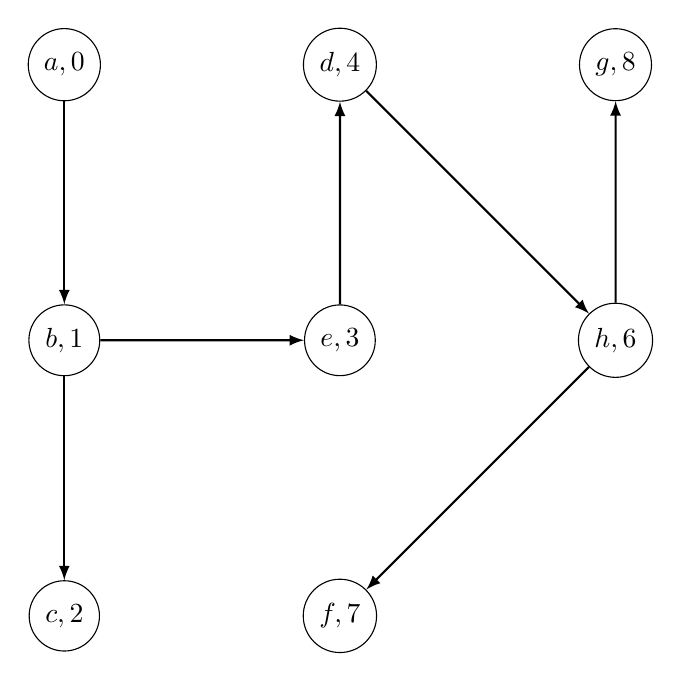
\begin{tikzpicture}[scale=3.5]
        % Noder
        \node[circle, draw] (a) at (0,2) {$a,0$};
        \node[circle, draw] (b) at (0,1) {$b,1$};
        \node[circle, draw] (c) at (0,0) {$c,2$};
        \node[circle, draw] (d) at (1,2) {$d,4$};
        \node[circle, draw] (e) at (1,1) {$e,3$};
        \node[circle, draw] (f) at (1,0) {$f,7$};
        \node[circle, draw] (g) at (2,2) {$g,8$};
        \node[circle, draw] (h) at (2,1) {$h,6$};

        % Kanter
        \draw[thick, -latex]  (a) to node[midway, above]  {} (b);
        \draw[thick, -latex]  (b) to node[midway, above]  {} (e);
        \draw[thick, -latex]  (b) to node[midway, above]  {} (c);
        \draw[thick, -latex]  (e) to node[midway, above]  {} (d);
        \draw[thick, -latex]  (d) to node[midway, above]  {} (h);
        \draw[thick, -latex]  (h) to node[midway, above]  {} (g);
        \draw[thick, -latex]  (h) to node[midway, above]  {} (f);
    \end{tikzpicture}
    \caption{Directed tree $T$ for $S$}
\end{figure}

\subsection[]{}



\subsection[]{}



\subsection[]{}



\end{document}